% ******************************************************** %
%              TEMPLATE DE INFORME ORGA2 v0.1              %
% ******************************************************** %
% ******************************************************** %
%                                                          %
% ALGUNOS PAQUETES REQUERIDOS (EN UBUNTU):                 %
% ========================================
%                                                          %
% texlive-latex-base                                       %
% texlive-latex-recommended                                %
% texlive-fonts-recommended                                %
% texlive-latex-extra?                                     %
% texlive-lang-spanish (en ubuntu 13.10)                   %
% ******************************************************** %


\documentclass[a4paper]{article}
\usepackage[spanish]{babel}
\usepackage[utf8]{inputenc}
\usepackage{charter}   % tipografia
\usepackage{graphicx}
%\usepackage{makeidx}
\usepackage{paralist} %itemize inline

%\usepackage{float}
%\usepackage{amsmath, amsthm, amssymb}
%\usepackage{amsfonts}
%\usepackage{sectsty}
%\usepackage{charter}
%\usepackage{wrapfig}
%\usepackage{listings}
%\lstset{language=C}
\usepackage{caption}

% \setcounter{secnumdepth}{2}
\usepackage{underscore}
\usepackage{caratula}
\usepackage{url}
\usepackage[document]{ragged2e}
\usepackage[export]{adjustbox}
\usepackage{subcaption}
\usepackage{floatrow}


% ********************************************************* %
% ~~~~~~~~              Code snippets             ~~~~~~~~~ %
% ********************************************************* %

\usepackage{color} % para snipets de codigo coloreados
\usepackage{fancybox}  % para el sbox de los snipets de codigo

\definecolor{litegrey}{gray}{0.94}

\newenvironment{codesnippet}{%
	\begin{Sbox}\begin{minipage}{\textwidth}\sffamily\small}%
	{\end{minipage}\end{Sbox}%
		\begin{center}%
		\vspace{-0.4cm}\colorbox{litegrey}{\TheSbox}\end{center}\vspace{0.3cm}}



% ********************************************************* %
% ~~~~~~~~         Formato de las páginas         ~~~~~~~~~ %
% ********************************************************* %

\usepackage{fancyhdr}
\usepackage{parskip}
\pagestyle{fancy}

%\renewcommand{\chaptermark}[1]{\markboth{#1}{}}
\renewcommand{\sectionmark}[1]{\markright{\thesection\ - #1}}

\fancyhf{}

\fancyhead[LO]{Sección \rightmark} % \thesection\ 
\fancyfoot[LO]{\small{Luis Enrique Badell Porto, Nicolas Bukovits, Kevin Frachtenberg}}
\fancyfoot[RO]{\thepage}
\renewcommand{\headrulewidth}{0.5pt}
\renewcommand{\footrulewidth}{0.5pt}
\setlength{\hoffset}{-0.8in}
\setlength{\textwidth}{16cm}
%\setlength{\hoffset}{-1.1cm}
%\setlength{\textwidth}{16cm}
\setlength{\headsep}{0.5cm}
\setlength{\textheight}{25cm}
\setlength{\voffset}{-0.7in}
\setlength{\headwidth}{\textwidth}
\setlength{\headheight}{13.1pt}
\setlength{\parindent}{4em}
\setlength{\parskip}{\baselineskip}

\renewcommand{\baselinestretch}{1.1}  % line spacing

% ******************************************************** %


\begin{document}


\thispagestyle{empty}
\materia{Organización del Computador II}
\submateria{Primer Cuatrimestre de 2016}
\titulo{Trabajo Práctico 2}
\subtitulo{Procesamiento de imágenes con SIMD}
\integrante{Luis Enrique Badell Porto}{246/13}{luisbadell@gmail.com}
\integrante{Nicolas Bukovits}{546/14}{nicko_buk@hotmail.com}
\integrante{Kevin Frachtenberg}{247/14}{kevinfra94@gmail.com}
\grupo{Grupo: Yo no manejo el raiting, yo manejo un Rolls-Royce}
\maketitle

%{\small\textbf{\flushleft{Resumen}}\\
\abstract {En el siguiente trabajo pr\'actico, se busca analizar, estudiar y comprender el funcionamiento y rendimiento de la tecnolog\'ia
SIMD (Single Instruction Multiple Data) inclu\'ida en el sistema SSE de los procesadores Intel. Para esto, se realizaron tres filtros
de im\'agenes (Cropflip, Sepia y Low Dynamic Range) en lenguaje C y en lenguaje ensamblador para aplicar sobre imagenes BMP, y luego se comparó el rendimiento entre ellos.
Los resultados obtenidos de estos experimentos, fueron plasmados y analizados en este informe.
}

%\newpage

%\thispagestyle{empty}
%\vfill


\thispagestyle{empty}
\vspace{3cm}
\tableofcontents
\newpage


%\normalsize
\newpage



\section{Introduccion}
\subsection{Cropflip}
El filtro cropflip recibe como parametros extra dos tamaños y dos offset. Un tamaño y un offset para las filas, y los otros dos para las columnas.
Lo que se hace con esto es recortar la imagen original en una nueva imagen e invertirla verticalmente. La imagen se recorta desde
donde los offsets lo indican hasta el tamaño indicado.
\newline 
Ejemplo: cropflip lena32.bmp 128 128 40 50 

\begin{figure}[!ht]
    \centering
    \begin{floatrow}
      \ffigbox[\FBwidth]{\caption{Antes del filtro cropflip}}{%
        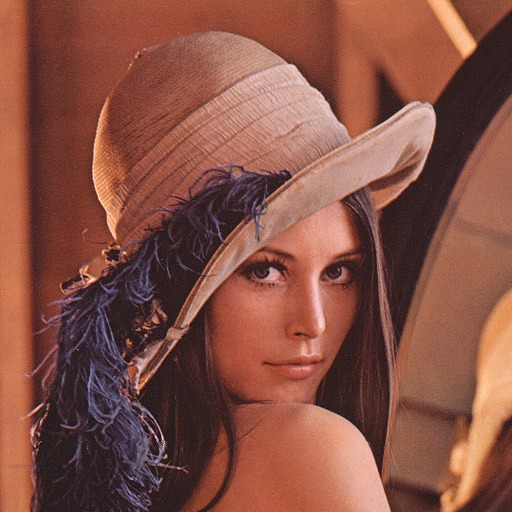
\includegraphics[scale=.25]{./imagenes/lena32.jpg}   
      }
      \ffigbox[\FBwidth]{\caption{Después del filtro cropflip}}{%
       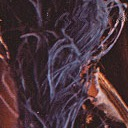
\includegraphics[scale=.5]{./imagenes/lena32-cropflip.jpg} 
      }
    \end{floatrow}
\end{figure}

Para el caso de la implementación en lenguaje C, se toma pixel por pixel y se copia al lugar correspondiente (invirtiendo la imagen)
en la imagen destino.
Por otro lado, en el caso de la implementación en lenguaje ensamblador, se utilizan los registros XMM para leer y copiar de a 4 pixels
en la imagen final.

\subsection{Sepia}
El filtro sepia, es el conocido filtro de imagenes que simula una foto antigüa. Para lograr este efecto, lo que se hace es una suma
de los canales de color (R, G, B. Llamaremos a esta suma ``SumaRGB'') y luego se multiplica por un valor fijo para cada canal (0.5 para el canal R, 0.3 para el G
y 0.2 para el canal B). Luego, manteniendo la transparencia en caso de haber, el pixel quedaría conformado por A = A, R = SumaRGB*0.5
, G = SumaRGB*0.3 y B = SumaRGB*0.2. \newline
Al igual que en Cropflip, en el caso de C, se trabaja pixel por pixel, mientras que en el caso del lenguaje ensamblador se trabaja un poco diferente:
Si bien se lee de a 4 pixeles de la imagen original, luego es necesario trabajar pixel por pixel ya que cada canal tiene un tamaño de 1 byte
y si quisiéramos realizar la suma de los 3 canales de los 4 pixeles en un solo registro, ésta no entraría en un byte. De esta forma, lo que se hace
es expandir (unpack) cada pixel para que cada canal pase a tener un tamaño de word (2 bytes). Así, la suma máxima será de 255 + 255 + 255, y esto sí
entra en un espacio de tamaño word. Sin embargo, las instrucciones que provee el procesador Intel para multiplicar por floats, nos obliga
a realizar otra expanción (unpack) de cada pixel, pero esta vez de word a Double word (4 bytes, mismo tamaño que un float).
Una vez están listos los cálculos de cada uno de los 4 pixels, se realizan 2 packs para llevar cada canal de doubleword a byte nuevamente.
\newline
Ejemplo: sepia foto.bmp
\begin{figure}[!ht]
    \centering
    \begin{floatrow}
      \ffigbox[\FBwidth]{\caption{Antes del filtro sepia}}{%
        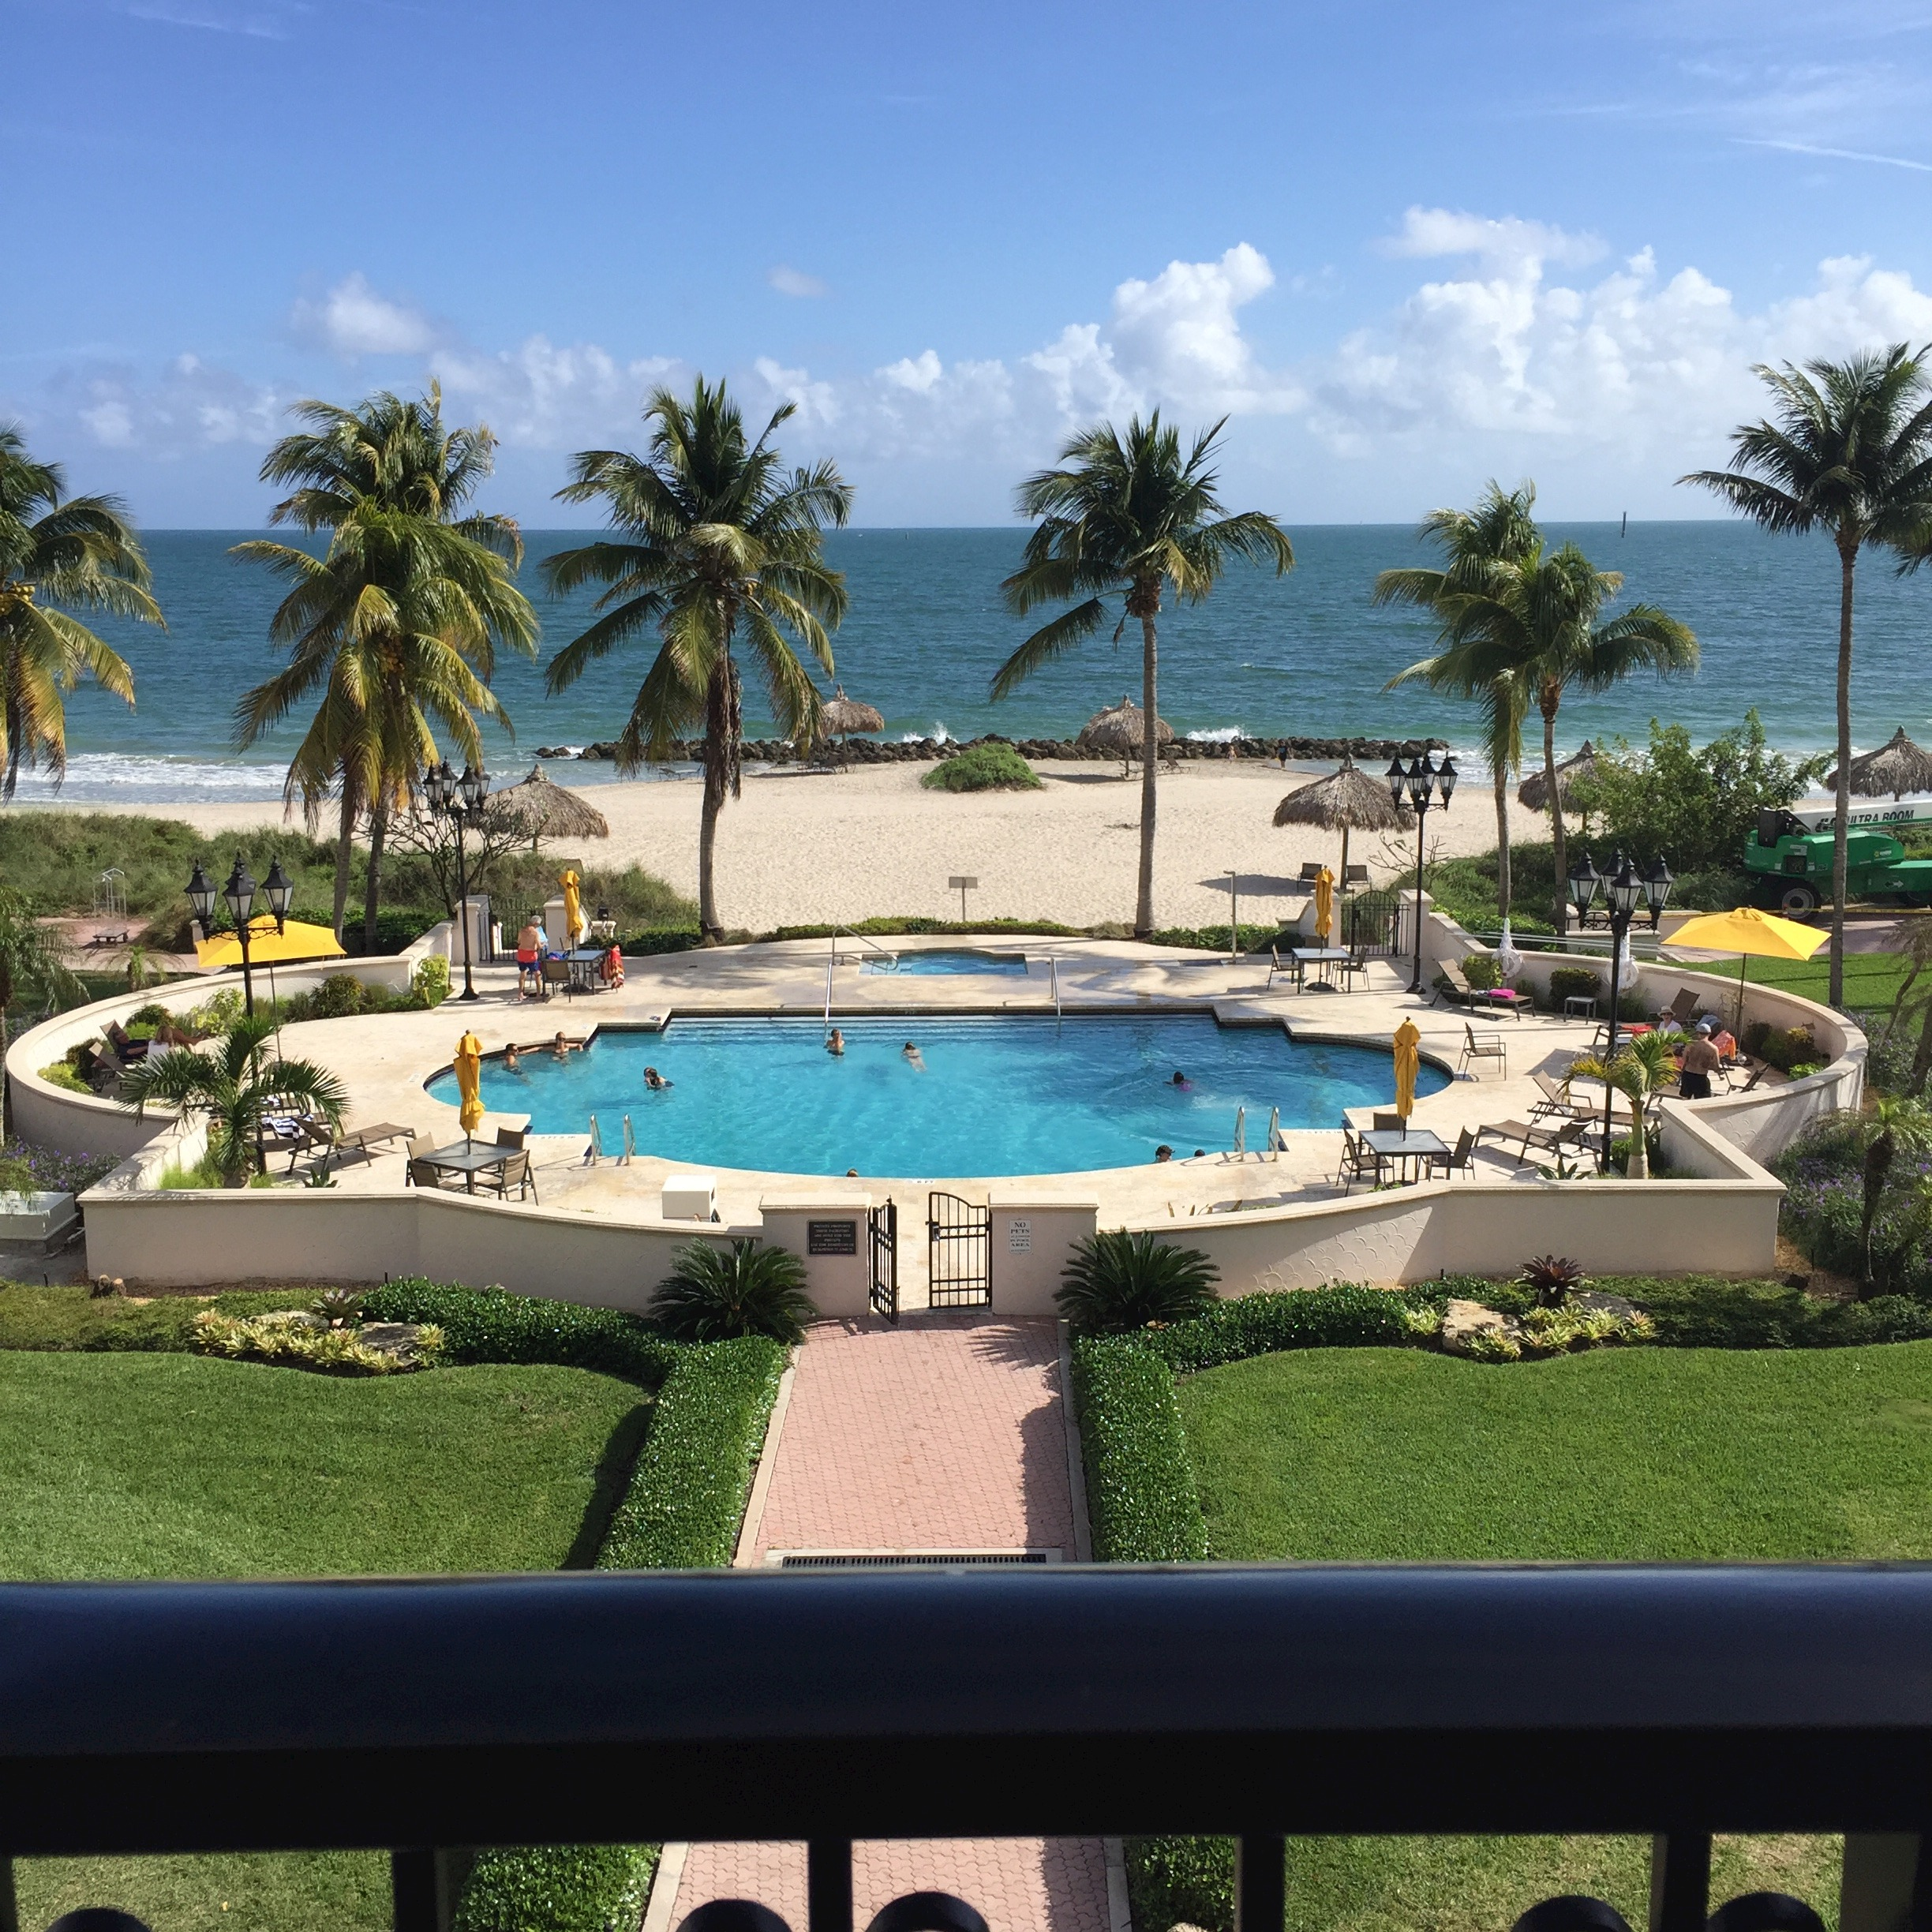
\includegraphics[scale=.04]{./imagenes/foto.jpg}   
      }
      \ffigbox[\FBwidth]{\caption{Después del filtro sepia}}{%
       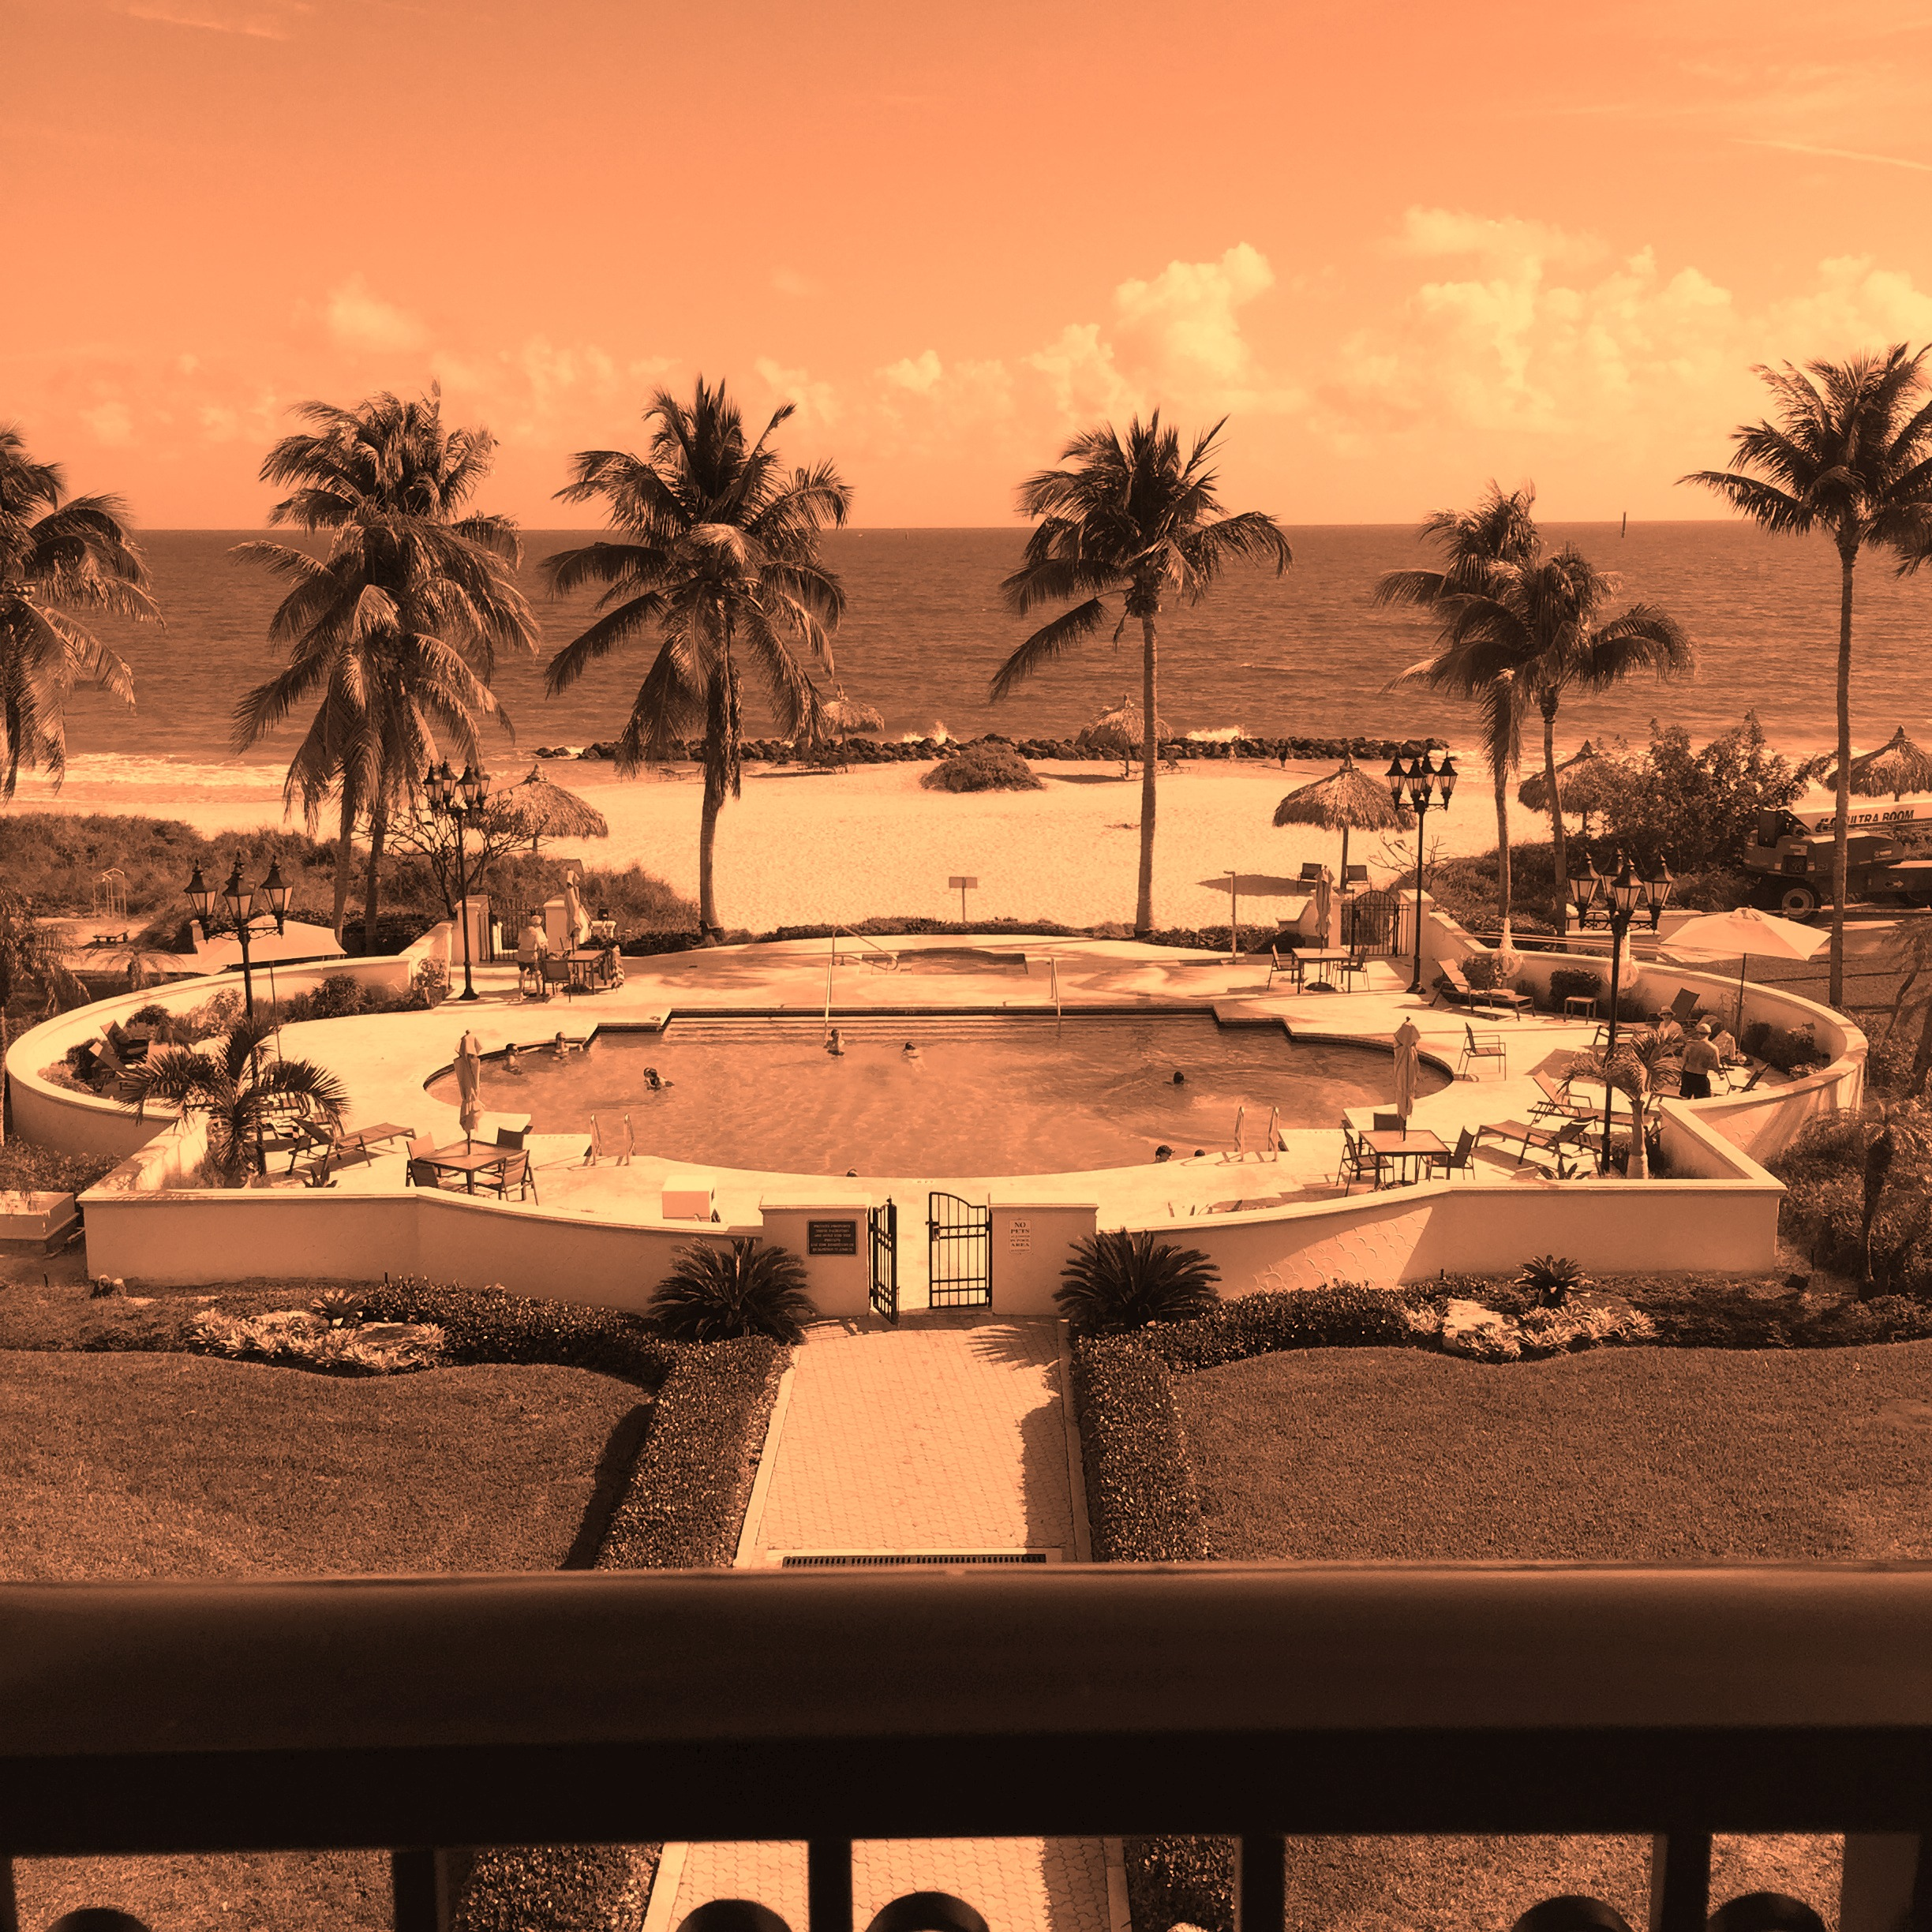
\includegraphics[scale=.04]{./imagenes/foto-sepia.jpg} 
      }
    \end{floatrow}
\end{figure}

\subsection{Low Dynamic Range}
Este filtro, más conocido como LDR, se logra realizando una serie de cálculos en base a los 25-vecinos de cada pixel del interior
de la imagen (si tomamos ``interior'' como 2 pixels hacia adentro desde cada borde) y un $\alpha$ pasado por parámetro, el cual puede ser
un valor entre -255 y 255. Lo que hace es agregar o quitar luminosidad dependiendo de este $\alpha$. El método para lograr este efecto es
modificar cada canal de color (R,G,B) del pixel a revisar, a través de realizar una suma de los 3 canales de color de los 25-vecinos del pixel a editar (incluyendo el mismo pixel),
luego se multiplica ese valor por el $\alpha$ y por el valor del canal del pixel en observación. Por último, se divide por un valor ``Max'',
que se da haciendo el cálculo del posible máximo del cálculo anterior (255*25*3*255), se suma el valor del canal antes multiplicado y antes
de guardarse, se satura a 0 y 255, que es el maximo de cada canal (ya que como el $\alpha$ puede ser negativo, es necesario tomar el caso
en que quede un número negativo en el canal).
\newline
El caso de C es igual a sepia y cropflip: Se analiza pixel por pixel. El caso del lenguaje ensamblador es parecido, ya que no se pueden
hacer cálculos tan grandes con 4 pixeles al mismo tiempo. Es por esto, que también se analiza pixel por pixel, pero para realizar el
cálculo de la suma de los 25 vecinos, las multiplicaciones, la división, suma y saturación, se utilizan instrucciones SSE.
\newline
Ejemplo: ldr bob.bmp 100
\begin{figure}[!ht]
    \centering
    \begin{floatrow}
      \ffigbox[\FBwidth]{\caption{Antes del filtro ldr}}{%
        
\includegraphics[scale=.25]{./imagenes/bob.jpg}   
      }
      \ffigbox[\FBwidth]{\caption{Después del filtro ldr}}{%
       
\includegraphics[scale=.25]{./imagenes/bob-ldr.jpg} 
      }
    \end{floatrow}
\end{figure}


\section{Desarrollo}

\subsection{Hipótesis y bases}
Nosotros tenemos como hipótesis que dadas las herramientas que nos ofrece la tecnología SSE, y que nosotros mismos somos los que nos
ocupamos de hacer una buena implementación en cada lenguaje, los algoritmos hechos en lenjuage ensamblador serán mucho más rápidos
que los que están hechos en lenguaje C. Sabemos que parte del retraso que tiene el lenguaje C se debe a que es el compilador quien decidirá cómo
optimizar el algoritmo implementado; esto es, traducir a código de máquina según la interpretación que le de el compilador al código C. Es por esto 
que usaremos el flag O3 como caso de compilación extra, y así poder comparar distintos métodos de compilación sobre una misma 
implementación del lenguaje C.
En cambio, para el caso del lenjuage ensamblador, es simplemente traducir a código de máquina, ya que son directamente las instrucciones
que el procesador deberá ejecutar.
\newline
Para poder comparar cada implementación de los filtros, los mismos se ejecután reiteradas veces en imagenes de distintos tamaños.
De cada ejecución, tomaremos el tiempo del clock antes de correr el programa y después de correrlo, y además observaremos
la cantidad de ciclos de reloj que toma cada vez. Si bien esto puede traer problemas como por ejemplo el tema de los \textit{outliers},
por razones de probabilidad y estadística, un promedio de cantidades grandes se acercará más a un promedio real.

\subsection{Implementación y Análisis}

\subsubsection{Cropflip}
Como se mencionó en la introducción, el filtro de Cropflip toma, en el caso de C, cada pixel y se copia de memoria a memoria. 
Sabemos que en la práctica esto solo funciona con un DMA, por lo que depende del compilador decidir cómo hacer las iteraciones para 
recorrer la imagen original y copiar cada pixel a la nueva posición de memoria.
Para el caso de ASM, se toma de a 4 pixels y se mueven a un registro XMM. dado que un pixel tiene tamaño de 32 bits y el tamaño
del registro XMM es de 128, hacer esto es posible mediante instrucciones SSE (en este caso, movdqu). Luego lo mueve nuevamente a memoria
en la posición correspondiente para ese pixel en la nueva imagen. 
Para este filtro, los tests que se realizaron consideraron distintos offsets y se realizaron sobre imágenes de distintos tamaños.
\newline
Los parámetros utilizados para esta experimentación fueron tamx: 128, tamy: 128, offsetx: i-128, offsety: i-128. Donde \textit{i} es
el tamaño de un lado de la imagen, que al ser cuadradas y múltiplos de 4, hace que sea indiferente el lado a elegir.
Este Offset permite tener en cuenta el desplazamiento que debe realizarse para empezar a copiar la imagen, el cual es hasta el último
bloque de 128x128 de la imagen original.
\newline
El primer caso de comparación es la implementación en C compilado sin el Flag O3 contra la implementación en ASM. En el siguiente gráfico
se puede observar la diferencia de tiempo de cada implementación en ciclos de reloj en función del tamaño de la imagen en pixels.

\begin{figure}[!ht]
    \centering
    \begin{floatrow}
      \ffigbox[\FBwidth]{\caption{Comparación C sin optimizar vs ASM}}{%
        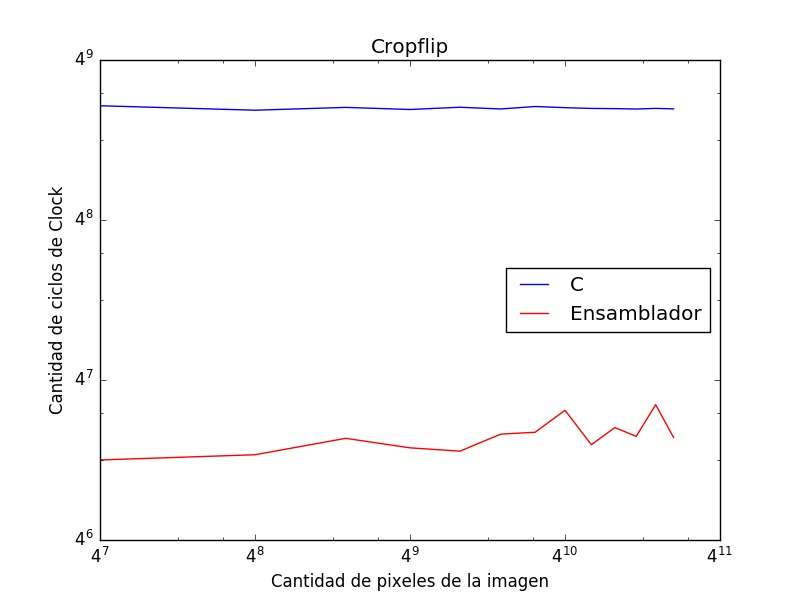
\includegraphics[scale=.25]{./imagenes/Cropflip0.jpeg}%cropflip-asmVSc.jpeg}   
      }
    \end{floatrow}
\end{figure}

Podemos observar de este experimento que la implementación en C es que si bien está basada en la misma idea que la implementación en ASM,
el código generado por el compilador hace que tome mucho más tiempo resolver cada aplicación del filtro hasta el punto de crecer linealmente
respecto del tamaño de la imágen. Podemos entender esto como una muestra de la diferencia en capacidad de procesamiento de los procesadores que utilizan
la tecnología SSE contra los que no la utilizan o no tienen.

\begin{figure}[!ht]
    \centering
    \begin{floatrow}
      \ffigbox[\FBwidth]{\caption{Comparación C con optimización O3 vs ASM}}{%
        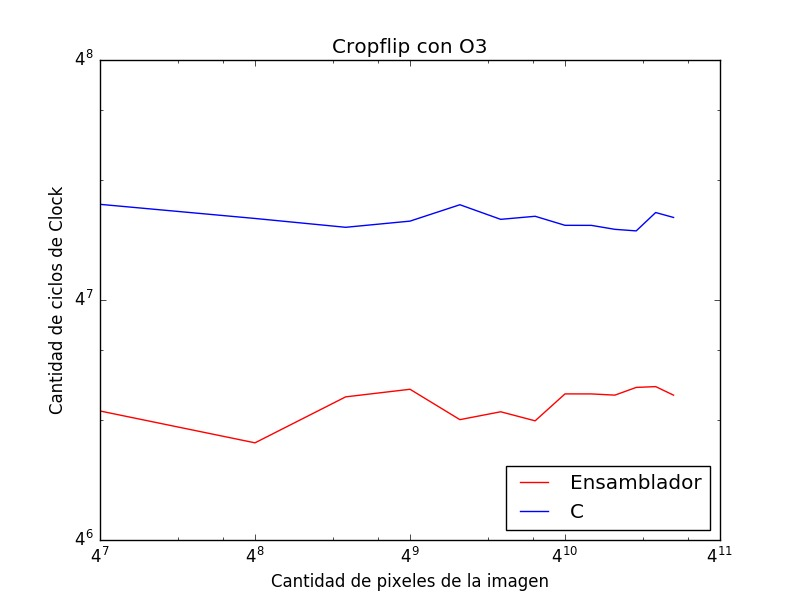
\includegraphics[scale=.25]{./imagenes/Cropflip3.jpeg}%cropflip-asmVScO3.jpeg}   
      }
    \end{floatrow}
\end{figure}

En este segundo experimento, comparamos la misma implementación C que el caso anterior pero esta vez compilado con el flag O3, 
el cual permite compilar el código utilizando tecnología SSE. Si bien se puede observar una amplia mejora respecto de la versión
sin el flag O3, aún se nota mucha diferencia en comparación con la versión de ASM.
\newline

En el siguiente cuadro comparativo se utilizó también el flag que permite utilizar tecnología AVX, el cual contiene acceso
a registros de 256-bits. A pesar de esto, no hubo una mejora de rendimiento respecto de la compilación sin el flag AVX.
\begin{figure}[!ht]
    \centering
    \begin{floatrow}
      \ffigbox[\FBwidth]{\caption{Comparación C con optimización O3 y AVX vs ASM}}{%
        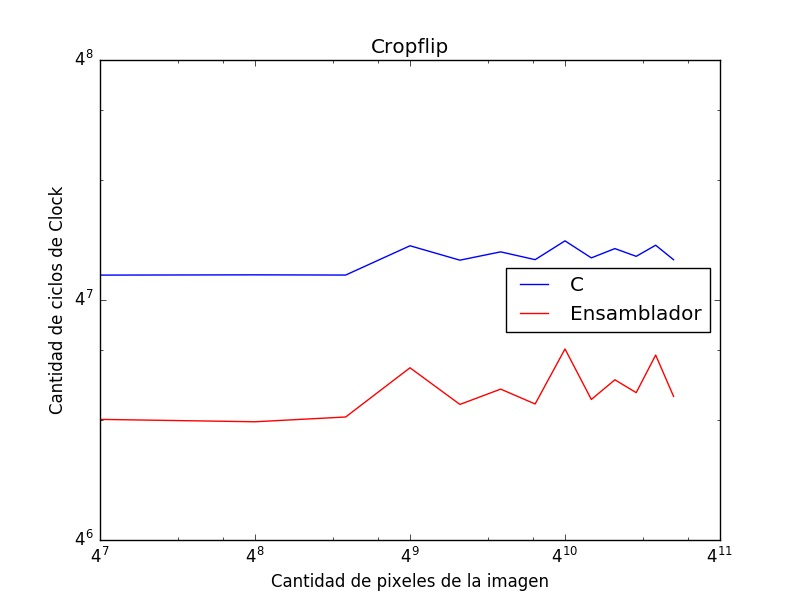
\includegraphics[scale=.25]{./imagenes/cropflip-asmVScO3AVX.jpeg}   
      }
    \end{floatrow}
\end{figure}


\subsubsection{Sepia}
Para el caso del filtro sepia, la implementación realizada en C consiste en lo siguiente: recorrer la matriz entera de pixeles(imagen), y por cada uno calcular la suma de los tres canales. Luego multiplicamos la suma de los canales por 0.5, y al mínimo valor entre éste y 255 se lo asignamos al canal rojo del nuevo pixel de la imagen a generar. La misma suma la multiplicamos por 0.3, calculamos el mínimo entre éste valor y 255, y finalmente se lo asignamos al canal verde del nuevo pixel. El mismo procedimiento se repite para el canal azul pero se multiplica el valor por 0.2. La transperencia se copia de manera exacta en el pixel del destino. La implementación realizada en lenguage ensamblador consiste en traerse cuatro pixeles de por vez, lo que permite reducir la cantidad de accesos a memoria. Luego, por cuestiones de tamaños, no es posible trabajar en paralelo con los 4 pixeles, ya que hay que realizar la suma de todos los canales de los mismos, lo cual no es posible representar el valor máximo que puede llegar a dar esta suma en 8 bits, que es el tamaño de cada canal. Por eso fue necesario expandir los 8 bits de cada canal a 16 bits, por lo cual sólo podiamos trabajar con 2 pixeles en paralelo. Luego de realizada la suma de los canales de los 2 pixeles, se tuvo que convertir el tipo de dato entero a float, lo que también produjo otra expansión del tamaño de los datos de 16 bits a 32 bits ya que es el tamaño requerido para trabajar con floats y poder realizar las multiplicaciones por 0.5,0.3 y 0.2 en cada caso particular. Para realizar las multiplicaciones se tuvo que hacer de a pixel por vez, debido a los 32 bits requeridos por cada canal. Luego se empaquetaron todos los resultados de los 4 pixeles individualmente, con cada canal en word, en un único registro, el cual se copia a memoria para poder copiar de a 4 pixeles. Básicamente, la mayor ganancia con esta implementación realizada en assembler, respecto de C, es que se leen y graban de a 4 pixeles por vez. 
\newline
Para el caso de los expermientos, se corrieron varios tests sobre imágenes de distintos tamaños, que es la única variable que está en juego para este filtro ya que no recibe ningún parámetro adicional.
\newline
El primer caso de comparación es la implementación en C, sin usar ninguna optimización en la compilación, contra la implementación en ASM.

%\begin{figure}[!ht]
%    \centering
%    \begin{floatrow}
%      \ffigbox[\FBwidth]{\caption{Comparación C sin optimización vs ASM}}{%
%        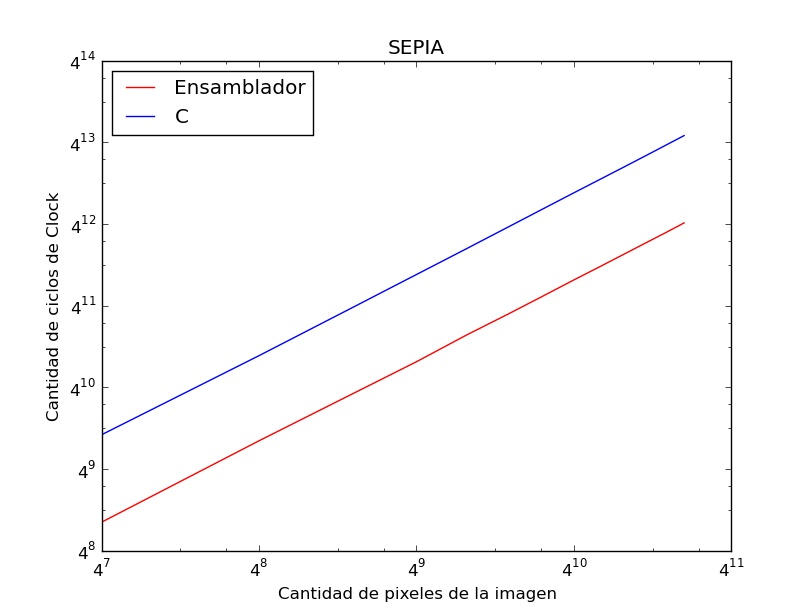
\includegraphics[scale=.25]{./imagenes/sepia-asmVSc.jpeg}   
%      }
%    \end{floatrow}
%\end{figure}

\noindent%
\begin{minipage}{\linewidth}% to keep image and caption on one page
\makebox[\linewidth]{%        to center the image
  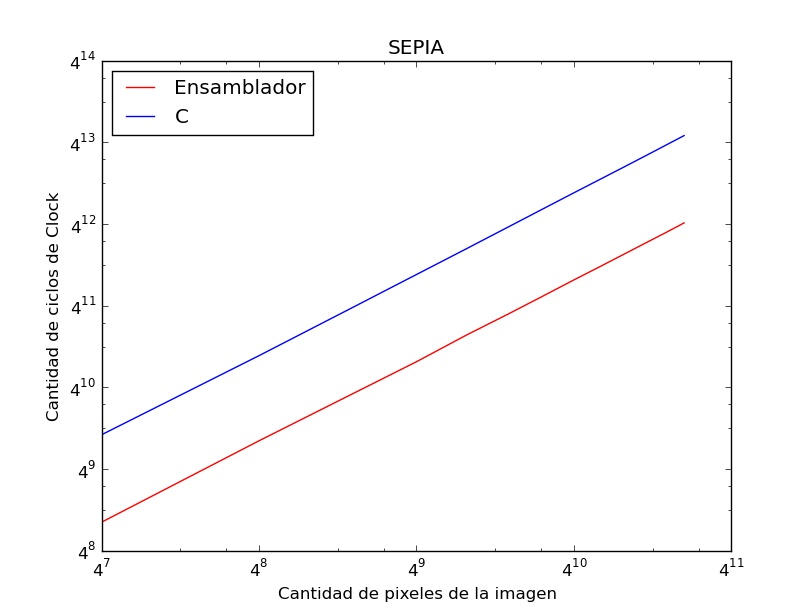
\includegraphics[keepaspectratio=true,scale=0.25]{./imagenes/sepia-asmVSc.jpeg}}
\captionof{figure}{Comparación C sin optimización vs ASM}%\label{visina8}%      only if needed  
\end{minipage}
\ \

Se puede observar claramente una relación lineal entre el tamaño de la imágen y el tiempo de procesamiento en ambas implementaciones, lo cual resulta intuitivo debido a los algoritmos utilizados. También se aprecia una brecha entre el tiempo que tomó correr los expermientos en C y Assembler, resaltando que los expermientos en assembler requirieron menos ciclos de clock para procesarse. Esta diferencia era la esperada, debido principalmente a la reducción de accesos a memoria gracias a la utilización de SSE en el código de Assembler. Se compararon las mismas implementaciones pero usando diferentes flags de optimizaciones para que realizara el compilador de C. Los resultados son los que arrojan los siguientes gráficos:

%\begin{figure}[!ht]
%    \centering
%    \begin{floatrow}
%      \ffigbox[\FBwidth]{\caption{Comparación C con flag O3 vs ASM}}{%
%        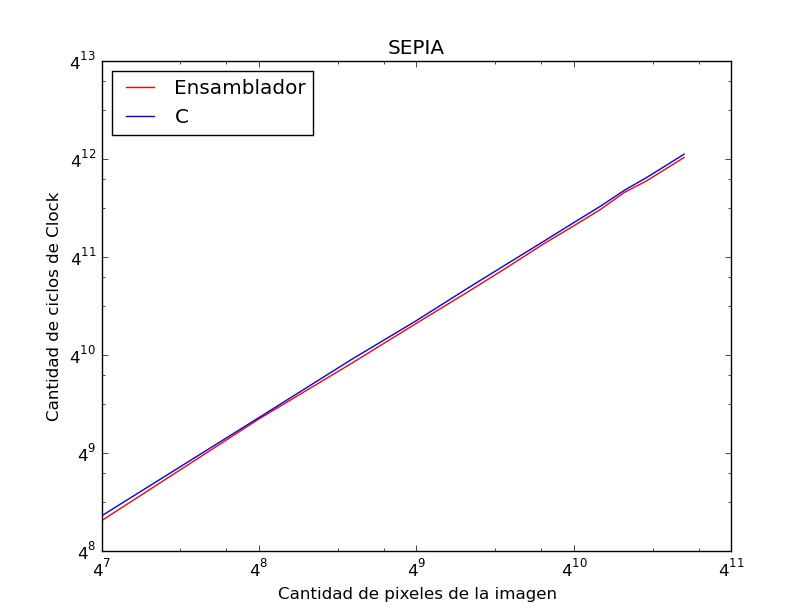
\includegraphics[scale=.25]{./imagenes/sepia-asmVScO3.jpeg}   
%      }
%    \end{floatrow}
%\end{figure}

\noindent%
\begin{minipage}{\linewidth}% to keep image and caption on one page
\makebox[\linewidth]{%        to center the image
  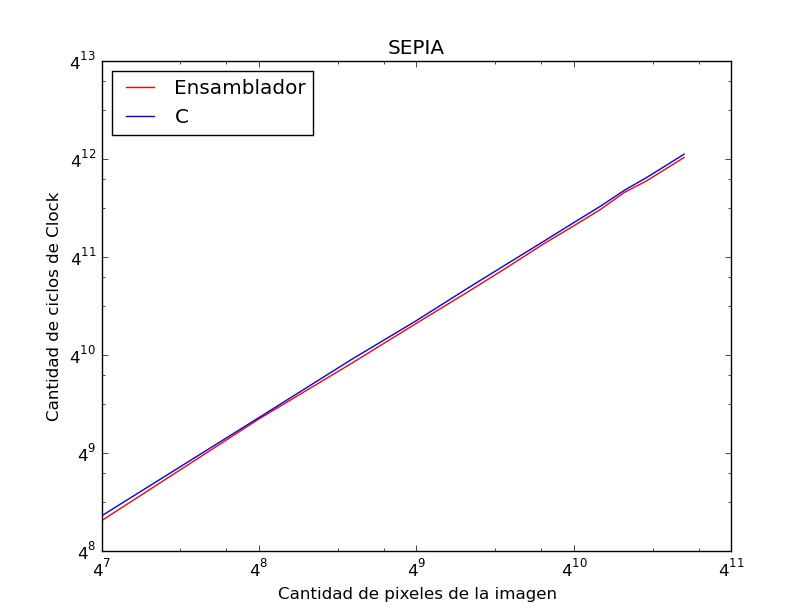
\includegraphics[keepaspectratio=true,scale=0.25]{./imagenes/sepia-asmVScO3.jpeg}}
\captionof{figure}{Comparación C con flag O3 vs ASM}%\label{visina8}%      only if needed  
\end{minipage}
\ \

Al utilizar el flag de optimización O3, el código generado por el compilador fue mucho más eficiente. Se observa en el gráfico una notable disminución de los tiempos de ejecución del código realizado en C, el cual casi iguala a la performance del realizado en ASM.

%\begin{figure}[!ht]
%    \centering
%    \begin{floatrow}
%      \ffigbox[\FBwidth]{\caption{Comparación C con flag O3 y mavx vs ASM}}{%
%        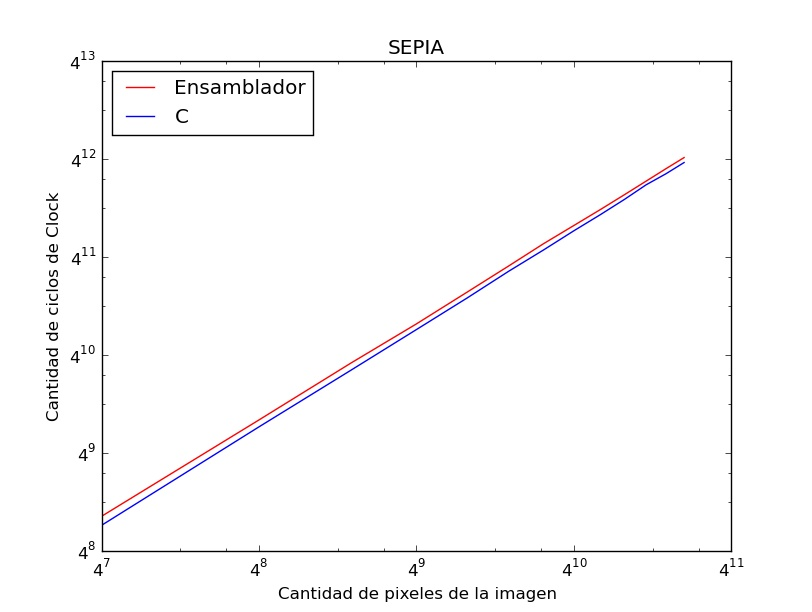
\includegraphics[scale=.25]{./imagenes/sepia-asmVScO3SSE4-2AVX.jpeg}   
%      }
%    \end{floatrow}
%\end{figure}

\noindent%
\begin{minipage}{\linewidth}% to keep image and caption on one page
\makebox[\linewidth]{%        to center the image
  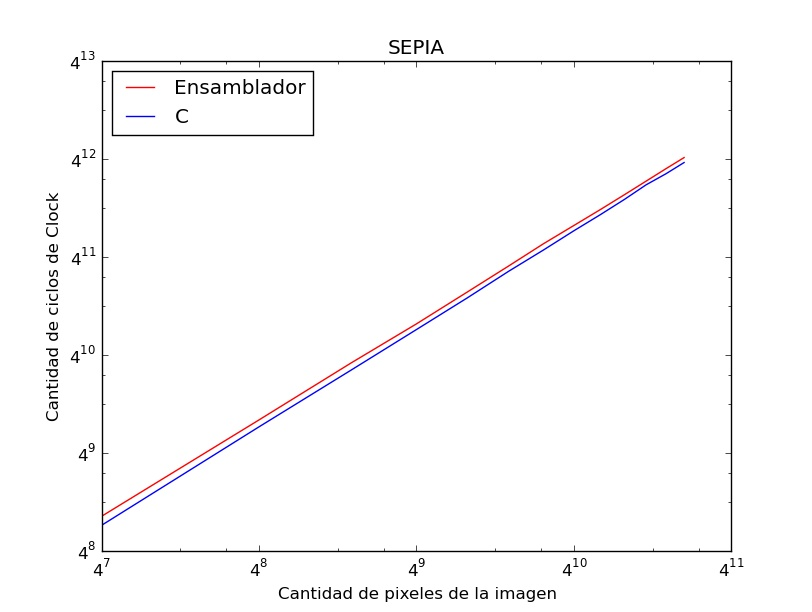
\includegraphics[keepaspectratio=true,scale=0.25]{./imagenes/sepia-asmVScO3SSE4-2AVX.jpeg}}
\captionof{figure}{Comparación C con flag O3 y mavx vs ASM}%\label{visina8}%      only if needed  
\end{minipage}
\ \

Este fue el resultado más interesante. Al compilar con la opción de AVX, que es una tecnología con nuevas instrucciones y expande los registos de 128 bits a 256 bits, se observa que el código generado por el compilador de C es ligeramente más óptimo en términos de tiempo de procesamiento que el realizado por nosotros en assembler. Era un resultado igualmente esperable, ya que al utilizar registros de 256 bits se reducen aún más los accesos a memoria necesarios para traer y guardar pixeles. La relación lineal entre tamaño de imagen y tiempo de procesamiento se mantiene nuevamente en el experimento.  

\subsubsection{Low Dynamic Range}
La idea específica de la implementación de este filtro tanto en C como en Assembler es ver pixel por pixel y realizar los cálculos 
de sus 25-vecinos por separado. Esto se hace de dos formas distintas dependiendo del lenguaje. 
\newline 
En el caso de C, primero se realiza la suma de los canales RGB de los 25-vecinos recorriendo pixel por pixel y canal por canal y 
eso se va guardando en una misma variable de tamaño int.
Esto hace que por cada pixel y por cada canal, se realice un acceso a memoria. \newline
Una vez obtenido la suma total, se la multiplica por el $\alpha$ pasado por parámetro. y se guarda en una nueva variable de tamaño Float.
Luego, esta nueva variable se la multiplica por separado por cada canal RGB del pixel a modificar y se guarda el resultado tres variables más
de tamaño Float. Después, se realiza la división por "Max", mencionado en la introducción de este informe y se le suma una vez más el canal
correspondiente a modificar del pixel central, guardando otra vez cada resultado en una nueva variable de tamaño Float. Finalmente, 
se satura cada variable y se la guarda en cada canal a modificar. Esto se hace una cantidad de veces igual a la cantidad total de pixels 
que tiene la imagen salvo por 2 líneas de pixeles en cada borde. Para ese caso, lo único que se hace es copiar los pixeles de la imagen original 
a la imagen destino. \newline
Para el caso de Assembler, lo que cambia respecto de la implementación C son la cantidad de accesos a memoria. Esto se corrige utilizando la 
tecnología SSE, con los registros de 128-bits, en los cuales al momento de realizar los cálculos de los 25-vecinos se cargan primero los 4 pixels
de cada fila y luego el último pixel de cada una. Además se utilizan instrucciones tales como \textit{phaddw} y \textit{paddw}, las cuales
perimten realizar sumas de datos empaquetados en los registros mencionado. Para el caso de la multiplicación y división, se utilizan las instrucciones
\textit{pmulld} y \textit{divps}, las cuales también trabajan con datos empaquetados en los registros de 128-bits. Para conservar el canal de 
transparencia, se utilizan las instrucciones \textit{pextrd}, la cual extrae un Double Word a un registro de 32 bits, y luego \textit{pinsrd}, 
la cual inserta de un registro de 32 bit un Double Word en un registro de 128 bits. Ambas instrucciones utilizan una máscara que indica cuál 
es el Double Word que se desea obtener o modificar.
\newline

En un primer experimento comparamos la implementación en C sin ningún tipo de optimización con la implementación en Assembler. En el gráfico 
resultante, se puede observar que ambas implementaciones crecen de manera lineal según el tamaño de la imagen. Sin embargo, la implementación en 
Assembler es aún más rápida que la de C.

\noindent%
\begin{minipage}{\linewidth}% to keep image and caption on one page
\makebox[\linewidth]{%        to center the image
  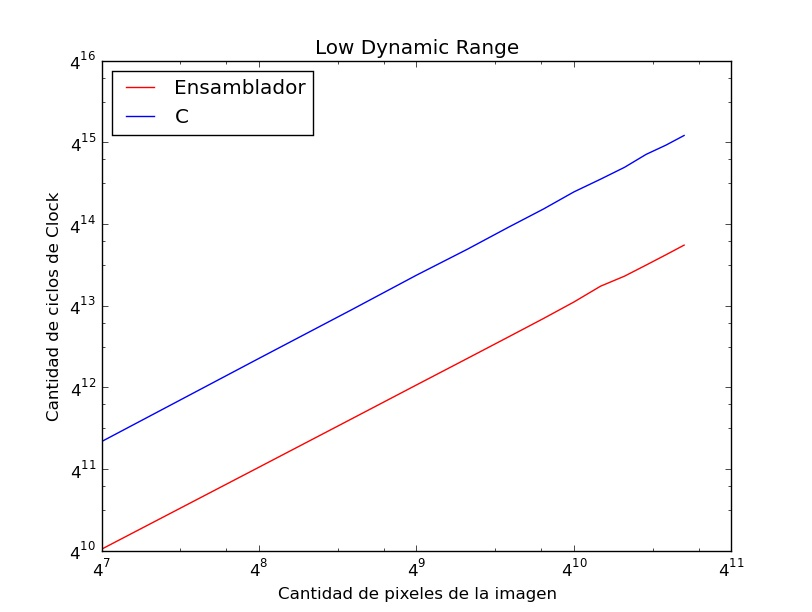
\includegraphics[keepaspectratio=true,scale=0.25]{./imagenes/ldr-asmVSc.jpeg}}
\captionof{figure}{Comparación C sin optimización vs ASM}%\label{visina8}%      only if needed  
\end{minipage}
\ \

En el segundo experimento, comparamos la implementación C compilando con el flag de optimización O3. A continuación se puede ver el gráfico del mismo:
\begin{figure}[!ht]
    \centering
    \begin{floatrow}
      \ffigbox[\FBwidth]{\caption{Comparación C con optimización O3 vs ASM}}{%
        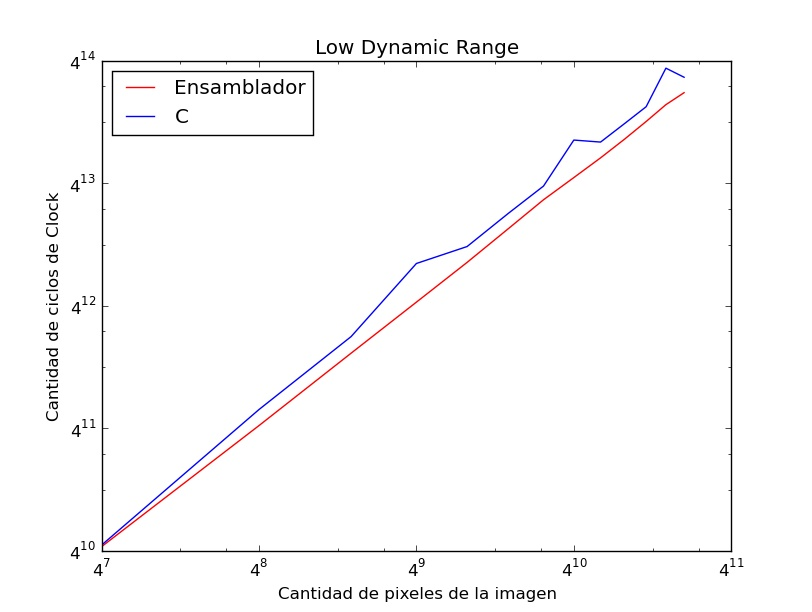
\includegraphics[scale=.25]{./imagenes/ldr-asmVScO3.jpeg}   
      }
    \end{floatrow}
\end{figure}
Podemos analizar en este caso que el flag O3 realmente cambia el rendimiento de la implementación. Si bien ya no es tán lineal como lo era en el
experimento anterior, ahora se acerca mucho al performance de la implementación en Assembler.
\newline
Como último experimento, agregamos el flag que permite utilizar los registros de 256 bits. Esta vez, se asemeja mucho al experimento anterior, pero
sigue siento un poco más rápido. El crecimiento de la cantidad de ciclos de procesador que toma, crece respecto del tamaño de la imagen de la misma
forma que sin el flag AVX.

\begin{figure}[!ht]
    \centering
    \begin{floatrow}
      \ffigbox[\FBwidth]{\caption{Comparación C con optimización O3 vs ASM}}{%
        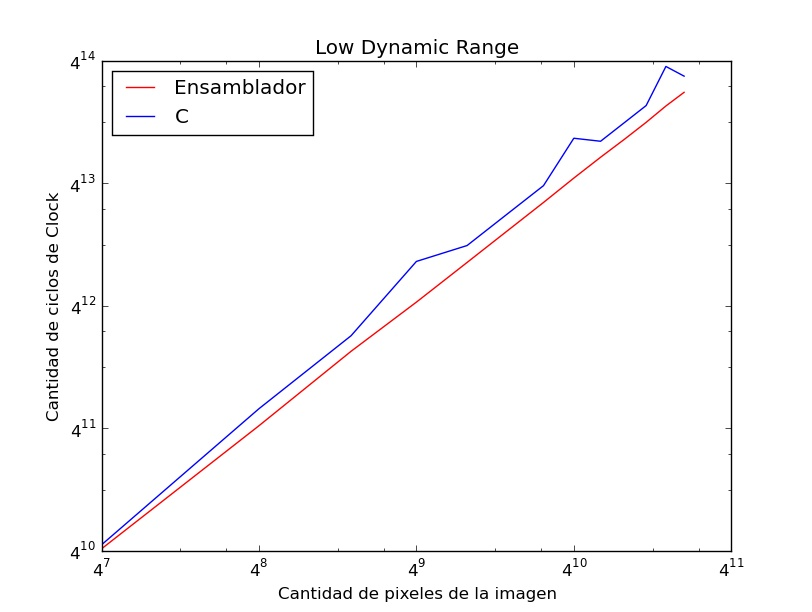
\includegraphics[scale=.25]{./imagenes/ldr-asmVScO3AVX.jpeg}   
      }
    \end{floatrow}
\end{figure}

\subsection{Comparación entre Compiladores}
Un compilador no es mas que un programa que basicamente toma el codigo C
y lo traduce a codigo de maquina. Existen varios para C, tales como como GCC (el cual se usa en gran parte de este trabajo), Clang y el Compilador de Intel.
Lo que hicimos en este experimento fue compilar los filtros con GCC y Clang en sus versiones 5.3.1 y 3.8.0 respectivamente, para luego realizar la comparación.
%Lo que vamos a hacer es compilar el codigo con Clang/GCC y ver si encontramos diferencias.Para comparar, se van a usar la version 4.8.4 de GCC y la 3.4 de Clang.
%Para realizar la comparacion, vamos a compilar el TP con GCC y luego con Clang.
%Para empezar, vamos a comparar con optimizacion nula
Nuestra hipótesis para este experimento es que el compilador de GCC optimiza más el código producido que Clang, ya que en caso contrario, este último estaría instalado por defecto
en muchos de los sistemas operativos existentes en lugar de GCC (teniendo en cuenta las muchas otras razones por las que puede no ser el caso).


Aqui el grafico de GCC sin optimización

\begin{figure}[H]
    \centering
    \begin{floatrow}
      \ffigbox[\FBwidth]{\caption{Filtros con GCC -O0}}{%
        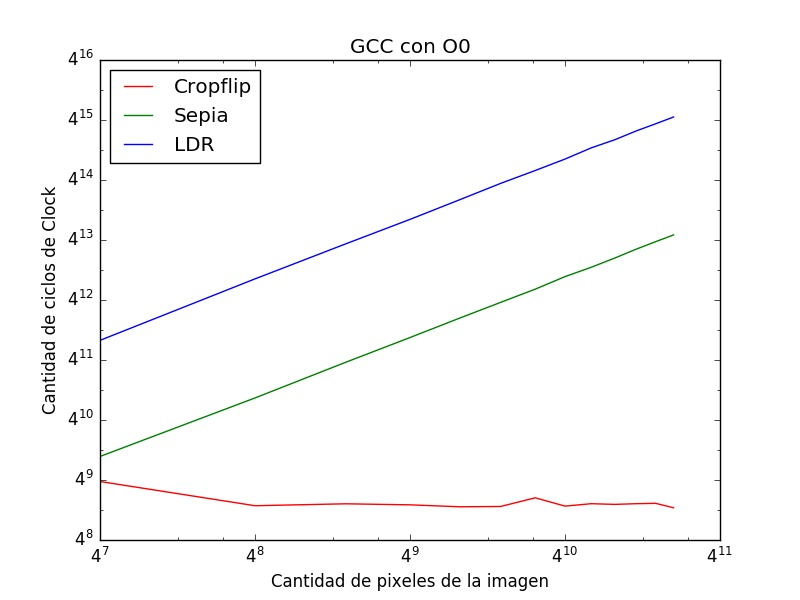
\includegraphics[scale=.55]{./imagenes/GCC0.jpg}
      }
    \end{floatrow}
\end{figure}


Aca vemos que Cropflip, que es el filtro más rápido, empieza tomando $4^9$ ciclos de reloj en la imagen más chica y finaliza cerca de la mitad entre $4^8$ y $4^9$.
Los otros dos filtros alcanzan hasta $4^{13}$ y $4^{15}$ ciclos de reloj.

Aqui el grafico de Clang

\begin{figure}[H]
    \centering
    \begin{floatrow}
      \ffigbox[\FBwidth]{\caption{Filtros con Clang -O0}}{%
        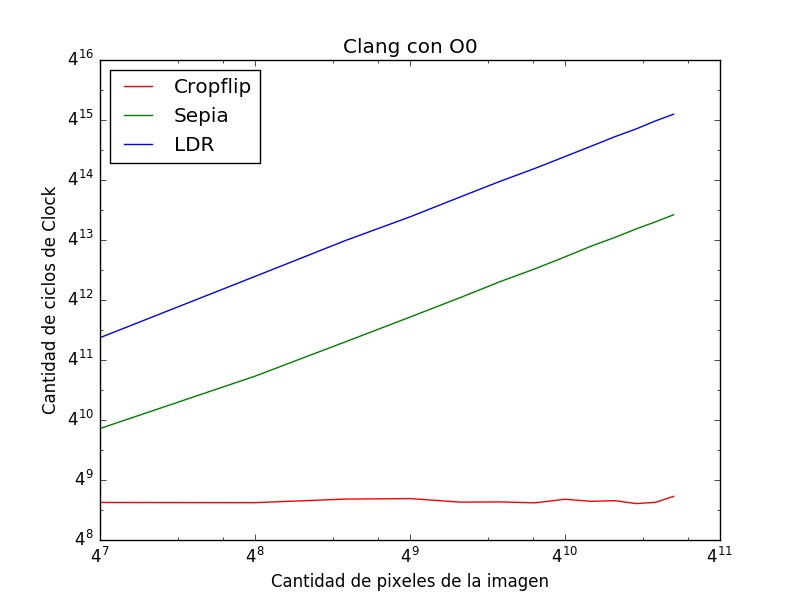
\includegraphics[scale=.55]{./imagenes/Clang0.jpg}
      }
    \end{floatrow}
\end{figure}

Tras este gráfico, observamos que las diferencias de LDR y Sepia son casi nulas entre los compiladores, sin embargo Cropflip tiene la diferencia de que es más
constante en cuanto a ciclos de reloj sobre tamaño de la imagen.


Ahora, vamos a repetir el mismo experimento pero variando las flags, esta vez vamos a usar 03. Como hipotesis, esperamos ver un comportamiento similar al visto en O0.
\begin{figure}[H]
    \centering
    \begin{floatrow}
      \ffigbox[\FBwidth]{\caption{Filtros con GCC -O3}}{%
        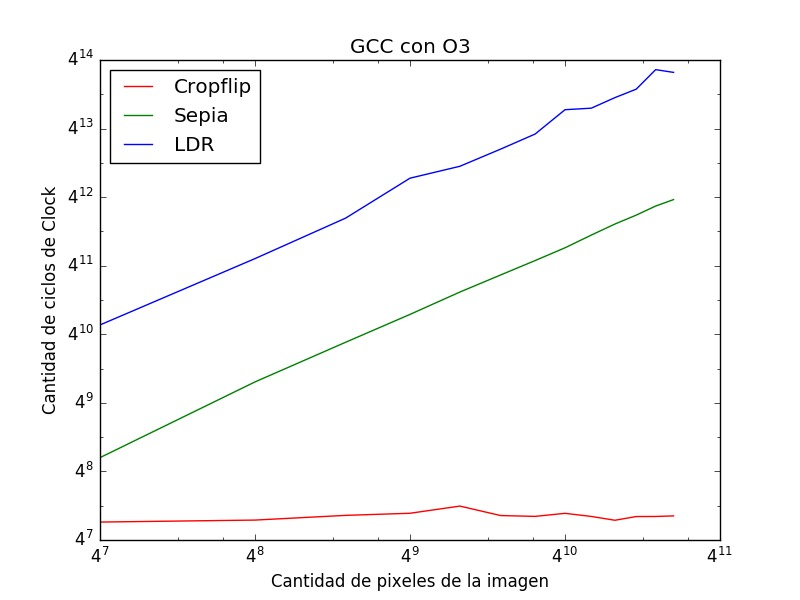
\includegraphics[scale=.55]{./imagenes/GCC3.jpg}
      }
    \end{floatrow}
\end{figure}


\begin{figure}[H]
    \centering
    \begin{floatrow}
      \ffigbox[\FBwidth]{\caption{Filtros con Clang -O3}}{%
        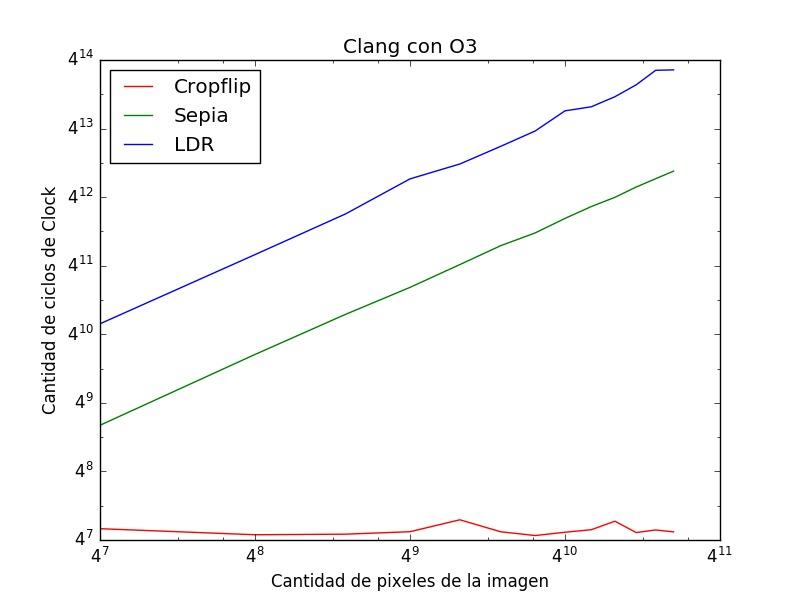
\includegraphics[scale=.55]{./imagenes/Clang3.jpg}
      }
    \end{floatrow}
\end{figure}

Ciertamente, se observó lo esperado. Tienen un comportamiento muy similar más allá de los flags de optimización. Podemos entender entonces que la desición
sobre usar un compilador u otro quedaría simplemente por preferencia y no por performance.


\section{Conclusiones y trabajo futuro}

Como conclusiones generales podemos destacar que los algoritmos implementados
en código Assembler con el uso de instrucciones SSE de Intel son más óptimos que
las implementaciones de los algoritmos en C (que se compilaron sin ningún 
tipo de optimización). Esto se debe principalmente a
su capacidad de procesar múltiples datos al mismo tiempo, generando un efecto
de paralelismo en el procesamiento y reduciendo la cantidad de accesos a memoria.
No obstante, al utilizar flags de optimización en la compilación de los algoritmos
implementados en C, la situación cambió en algunos expermientos. Para el caso particular del filtro sepia, resultó ligeramente más óptima en términos de tiempo de ejecución
la implementación en C, compilada con optimización O3 y para que utilize la tecnología AVX con registros de 256 bits, que la implemtación realizada en Assembler. Esto puede deberse a que al tener registros aún más grandes que los utilizados en Assembler (SSE de 128 bits), el código que generó el compilador permite procesar aún más datos en paralelo. 
Para el caso de Low Dynamic Range se notó una mejoría significativa usando la misma optimización pero que no alcanzó a igualar o superar al código realizado en Assembler. En el caso de Cropflip, la mejoría no fue significativa.
Por último, es importante destacar que el tiempo necesario para implementar un filtro en lenguaje Assembler es superior al del necesario para realizarlo en un lenguage de un nivel de abstración un poco más alto como es C. Si bien se observan diferencias significativas en la mayoría de los casos en cuestiones de performance, también conviene tener en cuenta el costo de implementación y analizar en cada caso y contexto de uso si el esfuerzo y tiempo adicional justifican los resultados, ya que como se mencionó antes, se puede obtener un muy buen resultado sólo usando optimizaciones del compilador en C.   

\par
Como siguientes pasos a realizar para este trabajo se pueden realizar diversas implementaciones de los filtros en el lenguaje Assembler para comparar su performance. Por ejemplo, para el caso de LDR, se podría realizar una implementación que además de trabajar con los 25 vecinos de un pixel con registros de 128 bits paralelamente, también se almacenen en registros de 128 bits las sumas parciales de estos 25 vecinos para que no haya que calcularlas todas nuevamente para el pixel próximo. La idea sería que solamente se tenga que computar lo que cambia, y lo que de alguna manera permanezca igual se puede almacenar. Esto reduciría los accesos a memoria y las operaciones a realizar, lo que supondría una mejora en el tiempo de ejecución que llevaría el filtro. Para el caso de sepia se podría probar con una implementación que en vez de realizar una multiplicación por un número decimal, realice una multiplicación por un entero y división por un entero para cada canal. Consideramos igualmente que esta implementación sería menos óptima en términos de ciclos de clock que la realizada actualmente. Para el caso de Cropflip no hay muchas formas de realizar la copia a memoria de la nueva imagen. Se podría probar con una implementación que recorra la imagen en otro orden o que la copie a memoria en otro orden, pero esto no supondría una diferencia significativa. Se podría usar instrucciones de la tecnología de AVX de Intel en caso de que el procesador lo admita, tanto para este último filtro como para todos. En el caso de usar la tecnología de AVX, todos las implementaciones deberían tener un tiempo de procesamiento menor que las anteriores, ya que con registros de 256 bits y nuevas instrucciones se pueden procesar aún más datos paralelamente.


%\begin{codesnippet}
%\begin{verbatim}

%struct Pepe {

 %   ...

%};

%\end{verbatim}
%\end{codesnippet}

\end{document}

